\section{ガサについて抗議すべき点}
\label{gasa_kogi}
	ガサの不当な点は大きく二つ, 「捜索自体の不当性」と「現場での不当行為」に分けられます. 以下の観点に基づいて寮生は抗議しています.

		\subsection{捜索自体の不当性について}
		 わかりやすい例を挙げると, 2013年にあった事案で, 「令状の捜索目的が熊野寮と無関係である」というようなことです. 寮生ではないし, 過去に住んでいたこともなければ, 立ち入ったこともない人物の被疑事件で令状が出されており, 自治会から抗議の声明を出していました.


    
    

		\subsection{現場での不当行為について}

			

			\subsubsection{過剰警備}

			\begin{wrapfigure}[18]{r}[1cm]{8cm}
				\centering
				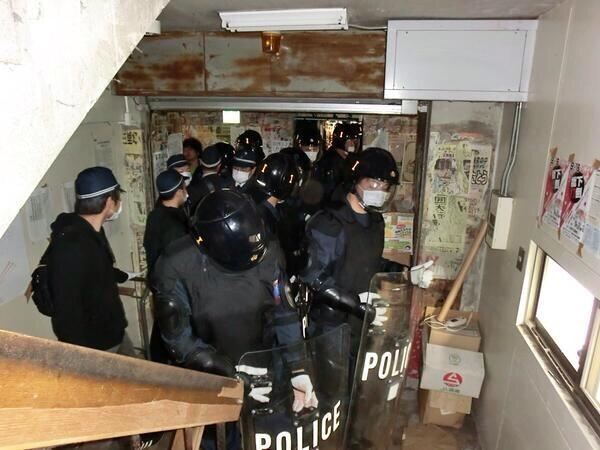
\includegraphics[width=7.8cm]{gazo/gasa.jpg}
				\caption*{\small{B棟1階階段周辺を占拠する機動隊}}
			\end{wrapfigure}

			捜索場所が1部屋のみで, 捜査員10名で足るような状況であっても, 50〜150名の機動隊を動員し, 玄関および捜索場所に至るまでの階段と廊下を不必要に占拠されるのが毎度のことです. 明らかに過剰な警備であり, 寮生の生活を不当に破壊するものとして抗議しています.
			
      
			\subsubsection{令状の不提示}
			令状を示すことなく押し入ることがあります. 本来は敷地に入る前に提示すべきものです. 2017年1月のガサで久しぶりに正門前での提示がありましたが, 2013年からそれまで正門前で提示されたことはありませんでした.

			\subsubsection{警察手帳不提示}
			「提示の必要はない」とはっきり言い放つ捜査員が度々現れますが, 人の住居を占拠しておきながら, 自身が警察官であることを示さなくてもよい, というのは一体どういうことなのでしょうか.

			「警察手帳規則第5条(証票及び記章の呈示) : 職務の執行に当たり, 警察官, 皇宮護衛官又は交通巡視員であることを示す必要があるときは, 証票及び記章を呈示しなければならない」に違反していると考えられます.

			\subsubsection{無関係な寮生の撮影}
			捜査員が, 廊下などの過剰警備に抗議する寮生や授業に出ていく寮生を終始撮影することがあります.

			警察官は捜査に際し, 捜査に関係の無いものを押収・撮影してはいけないとされています. よって, 公安警察の行為は肖像権の侵害にあたり, また, 憲法十三条をみても違憲行為であると考えられます. このような事例に関し, 捜査に無関係な第三者の撮影を違憲・違法とする最高裁の判例もあり, 言い逃れは不可能です.

			\subsubsection{2021年ガサでは機動隊は入構しなかった}
			2021年6月のガサでは正門前で寮生が警察に抗議した結果、機動隊は正門前で待機し、私服の捜査員のみが入構し捜索を行いました。\emphbf{機動隊が寮内で警備に当たらなくても、粛々と安全に捜索できることが証明される形になりました。}
			